% =============================================================================
% DOC-01 -- Scientific article, first full draft (IEEEtran conference).
% Project: SC-TPU + RV32I SoC on the Sipeed Tang Nano 9K (GW1NR-9).
% Author of this file: documentation-engineer.  Input revision: git eee3352.
%
% Build:  cd reports/article && latexmk -pdf -interaction=nonstopmode \
%                                        -halt-on-error main.tex
% Figures: vector PDFs generated by reports/figures/article_figures.py from
%          reports/sw/accuracy.json (log: logs/doc/article_figures.log);
%          block/timing diagrams are TikZ (this file).
%
% Number policy (CLAUDE.md, engineering-evidence skill):
%   * every number carries a "% evidence: <path>" comment on or next to its line;
%   * labels used in the text: SIMULATION, CALCULATION, SOURCE, ASSUMPTION;
%     no MEASUREMENT exists in this project (no hardware was operated);
%   * SC-TPU hardware numbers (RTL utilisation, Fmax, RTL bit-exactness,
%     measured CYCLES) do not exist yet: they are written as \TBD{name},
%     which prints a red [TBD:name].  All placeholders are listed in
%     reports/article/PLACEHOLDERS.md.
% =============================================================================
\documentclass[conference]{IEEEtran}

\usepackage[T1]{fontenc}
\usepackage{amsmath,amssymb}
\usepackage{graphicx}
\usepackage{cite}
\usepackage{booktabs}
\usepackage{multirow}
\usepackage{xcolor}
\usepackage{tikz}
\usetikzlibrary{positioning,arrows.meta,calc,fit,decorations.pathreplacing}
\usepackage{url}
\usepackage[hidelinks]{hyperref}

% Figures generated by scripts in reports/figures/.
\graphicspath{{../figures/}}

% -----------------------------------------------------------------------------
% Placeholder for numbers that do not exist yet (SC-TPU RTL still in progress;
% design change rev B pending).  Prints a red, bold [TBD:name].
% -----------------------------------------------------------------------------
\newcommand{\TBD}[1]{\textcolor{red}{\textbf{[TBD:\detokenize{#1}]}}}

% Small helpers for consistent notation.
\newcommand{\Dp}{D'}                 % post-processed accumulator (spec: Dp)
\newcommand{\NL}{N_{L}}              % neuron lanes
\newcommand{\IL}{N_{I}}              % input lanes
\newcommand{\lbl}[1]{\textsc{#1}}    % evidence label in running text

\begin{document}

\title{A Stochastic-Computing Tensor Unit and an RV32I Core on a 9K-LUT FPGA:\\
Bit-Exact Co-Design for Tiny-MLP Inference}

\author{\IEEEauthorblockN{\TBD{authors}}
\IEEEauthorblockA{\TBD{affiliation}}}

\maketitle

% =============================================================================
\begin{abstract}
Stochastic computing (SC) replaces a multiplier by a single logic gate acting
on random bit-streams, which makes it attractive for the smallest FPGAs, where
dedicated multipliers are scarce. We present the co-design of an SC tensor
processing unit (SC-TPU) and a multi-cycle RV32I processor for an 8640-LUT4
Gowin GW1NR-9 device (Sipeed Tang Nano 9K). The SC-TPU is a 16$\times$8
weight-stationary tile of bipolar XNOR multipliers with accumulative parallel
counters, driven by 8-step leap-forward LFSRs in three decorrelation modes.
Its behaviour, including the integer post-processing, is specified bit-exactly
so that a Python golden model, the training flow and the RTL must agree bit for
bit. For a 64-16-10 MLP on the 8$\times$8 digits set, simulation of the golden
model gives 95.0\,\% test accuracy for the expected-value (exact integer)
datapath and 94.4\,\% (95\,\% CI 91.6--96.4\,\%) for SC with independent
generators at stream length 256 (rev~A seeds); shared random numbers drop to 65.6\,\%. An
analytical variance model predicts the measured RMS stochastic error within a
factor 0.74--1.13. The CPU passes 44 ISS-checked programs under four bus timing
configurations (176/176 runs) and closes timing at 53.26\,MHz (worst of three
place-and-route seeds) against a 27\,MHz clock. All results are simulations
with an open-source flow; no hardware has been operated. SC-TPU implementation
figures are pending (\TBD{tpu-lut}, \TBD{soc-fmax-worst}).
% evidence: reports/sw/accuracy.json (EV 342/360; mode2 K8 340/360; mode0 K8 236/360)
% evidence: reports/sw/error_model.md (ratio 0.82-1.13, exception 0.74)
% evidence: logs/cpu/sim_cpu_summary.log ("# runs: 176 / 176 PASS")
% evidence: logs/cpu/pnr_s2.log (53.26 MHz); requirements/BUDGETS.md 1.1 (8640 LUT4, SOURCE S-001/S-027)
\end{abstract}

\begin{IEEEkeywords}
stochastic computing, neural network accelerator, RISC-V, FPGA, LFSR,
bit-exact golden model, open-source FPGA toolchain
\end{IEEEkeywords}

% =============================================================================
\section{Introduction}
\label{sec:intro}

Low-cost FPGAs with fewer than ten thousand look-up tables are widely used in
education, prototyping and small embedded products, but they offer only a
handful of hard multipliers. The GW1NR-9 device used here has 8640 LUT4
positions, 6480 flip-flops, 26 block RAMs and 20 18$\times$18
multipliers~\cite{sipeed_tn9k}.
% evidence: management/SOURCES.md S-001, S-002, S-005, S-010 (SOURCE, Sipeed wiki D-09 + chip database D-20)
A binary int8 neural-network datapath on such a device is limited to at most
40 hard 9$\times$9 multiply--accumulate (MAC) lanes, or must spend roughly 70
LUTs per soft 8$\times$8 multiplier (rough \lbl{calculation}).
% evidence: management/DECISIONS.md ADR-001 option B (~70 LUT soft multiplier, rough CALCULATION); management/SOURCES.md S-032 (40 MULT9X9, SOURCE D-20)

Stochastic computing~\cite{gaines1969,alaghi2013survey} encodes a number as the
probability of a one in a random bit-stream. A multiplication then reduces to
a single AND (unipolar) or XNOR (bipolar) gate, and the precision becomes a
run-time parameter: doubling the stream length $L$ halves the variance of the
result. Neural networks tolerate moderate arithmetic noise, which has made them
a prominent application of SC~\cite{brown2001stochastic,%
kim2016dynamic,ren2017scdcnn}. The price is latency ($L$ clock cycles per
product), the cost of random-number generation, and a sensitivity to
correlation between streams.

A second, less discussed difficulty is \emph{verification}: an SC result is a
random variable, so a hardware/software comparison is meaningless unless the
random sequence is defined as precisely as the arithmetic. This paper treats
the random-number generators, their seeding and their sequencing as part of a
bit-exact architectural contract.

\textbf{Contributions.}
\begin{enumerate}
\item A complete, small SoC architecture for the Tang Nano 9K: a multi-cycle
  RV32I CPU~\cite{riscv2019unpriv} orchestrating a 16$\times$8 weight-stationary
  bipolar SC tile with accumulative parallel counters (APC), using only an
  open-source flow~\cite{shah2019yosysnextpnr,yosys,apicula}
  (Section~\ref{sec:arch}).
\item A bit-exact specification of the SC datapath, including an 8-step
  leap-forward LFSR, three RNG decorrelation modes and integer
  post-processing, mirrored by a Python golden model used for
  quantisation-aware training with SC noise (Section~\ref{sec:method}).
\item An accuracy study versus stream length and RNG mode with 95\,\%
  confidence intervals and a seed ensemble, and an analytical variance model
  checked against simulation (Section~\ref{sec:results}).
\item A verification methodology with ISS-based differential testing of the
  CPU (44 programs $\times$ 4 bus timings) and fault-injection checks of the
  testbenches, and an explicit account of what remains unverified
  (Section~\ref{sec:discussion}).
  % evidence: logs/cpu/sim_cpu_summary.log
\end{enumerate}

% =============================================================================
\section{Background and Related Work}
\label{sec:background}

\subsection{Stochastic number encoding}
A stochastic number (SN) is a bit-stream $b_0,\dots,b_{L-1}$. In
\emph{unipolar} encoding it represents $p=P(b_k{=}1)\in[0,1]$; in
\emph{bipolar} encoding it represents $v = 2p-1 \in[-1,1]$, which admits signed
weights with a single stream per operand~\cite{gaines1969,alaghi2013survey}.
A stochastic number generator (SNG) converts a binary code $c$ into a stream by
comparing it with a pseudo-random number $r$: $b=[r<c]$. With $r$ uniform on
$\{0,\dots,2^n-1\}$, $P(b{=}1)=c/2^n$.

\subsection{Multiplication and accumulation}
For two independent unipolar streams the AND gate gives $P(a\wedge b)=p_ap_b$.
For bipolar streams the XNOR gate gives
\begin{equation}
  P\big(\overline{a\oplus b}=1\big) = \tfrac{1}{2}\left(1 + v_a v_b\right),
  \label{eq:xnor}
\end{equation}
i.e.\ the bipolar product~\cite{brown2001stochastic,alaghi2013survey}.
Accumulating many products with a multiplexer scales the sum down by the fan-in
and loses precision. An accumulative parallel counter instead counts the ones
of all product streams in each cycle and adds the count to a binary
accumulator, so the sum is exact in expectation and leaves the stochastic
domain; SC-DCNN~\cite{ren2017scdcnn} studied such APC-based inner products for
deep convolutional networks. Kim \emph{et al.}~\cite{kim2016dynamic} exploited
the stream length as a run-time energy--accuracy knob in deep networks.

\subsection{Precision, correlation and LFSRs}
An $L$-bit estimate of $p$ has variance $p(1-p)/L$, so every factor of four in
$L$ adds one bit of precision. Equation~\eqref{eq:xnor} holds only for
independent streams; streams generated from the same or from shifted random
sequences are correlated and bias or inflate the error~\cite{alaghi2013survey}.
Linear-feedback shift registers (LFSRs) are the usual cheap random source.
Taking $n$ consecutive bits of a single-step LFSR as $r$ yields successive
values that are shifted copies of each other, and two LFSRs with the same
polynomial produce lagged copies of the same maximal-length sequence. Both
effects matter in a small design that cannot afford many independent
generators.

\subsection{Small RISC-V cores and open FPGA flows}
PicoRV32~\cite{wolf_picorv32} is a size-optimised RV32 core with the same
native valid/ready memory interface that we adopt. The Yosys and nextpnr
tools~\cite{shah2019yosysnextpnr,yosys}, together with the reverse-engineered
Gowin database of Project Apicula~\cite{apicula}, provide a fully open flow for
the GW1N family; we use it exclusively.

% =============================================================================
\section{Architecture}
\label{sec:arch}

\subsection{SoC overview}
Fig.~\ref{fig:soc} shows the SoC. A single 27\,MHz clock domain is driven by
the board oscillator (no PLL); the reset button passes through a two-flip-flop
synchroniser into a synchronous active-high reset.
% evidence: design/architecture/ARCHITECTURE.md sec. 2; management/INTERFACES.json "clock"
The CPU is the only bus master. Slaves are selected by address bits [31:28]
(Table~\ref{tab:memmap}); an access to an unmapped region returns zero,
completes normally and sets a sticky debug flag, so a software error can never
hang the bus. The bus is a native valid/ready protocol: the master holds
\texttt{mem\_valid}, address, data and byte strobes stable until the slave
returns a one-cycle \texttt{mem\_ready} pulse.
% evidence: design/architecture/ARCHITECTURE.md sec. 3, 4

\begin{figure}[!t]
\centering
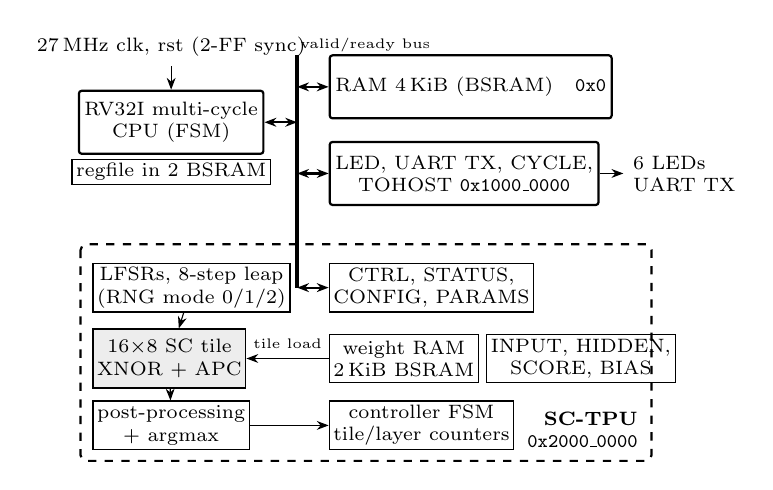
\begin{tikzpicture}[
    font=\scriptsize,
    blk/.style={draw, thick, rounded corners=1pt, align=center,
                minimum height=0.8cm, inner sep=2pt},
    sub/.style={draw, align=center, minimum height=0.62cm, inner sep=1.5pt,
                minimum width=1.75cm},
    >={Stealth[length=1.5mm]}]
  % ---- CPU (only bus master) -------------------------------------------
  \node[blk, minimum width=2.2cm] (cpu) at (1.1,0.35)
       {RV32I multi-cycle\\CPU (FSM)};
  \node[draw, align=center, minimum width=2.2cm, inner sep=1.5pt,
        below=0.05cm of cpu] (rf) {regfile in 2 BSRAM};
  \draw[<-] (cpu.north) -- ++(0,0.3) node[above]
       {27\,MHz clk, rst (2-FF sync)};
  % ---- Bus ----------------------------------------------------------------
  \draw[line width=1.6pt] (2.7,1.2) -- (2.7,-1.75);
  \node[anchor=south west, font=\tiny, inner sep=1pt] at (2.7,1.2) {valid/ready bus};
  \draw[<->, thick] (cpu.east) -- (2.7,0.35);
  % ---- RAM and peripherals ---------------------------------------------
  \node[blk, minimum width=2.75cm, anchor=west] (ram) at (3.1,0.8)
       {RAM 4\,KiB (BSRAM)\quad\texttt{0x0}};
  \node[blk, minimum width=2.75cm, anchor=west] (per) at (3.1,-0.3)
       {LED, UART TX, CYCLE,\\TOHOST \texttt{0x1000\_0000}};
  \draw[<->, thick] (2.7,0.8) -- (ram.west);
  \draw[<->, thick] (2.7,-0.3) -- (per.west);
  \draw[->] (per.east) -- ++(0.3,0) node[right, align=left]
       {6 LEDs\\UART TX};
  % ---- SC-TPU -------------------------------------------------------------
  \draw[thick, dashed, rounded corners=2pt] (-0.05,-1.2) rectangle (7.2,-3.95);
  \node[anchor=south east, font=\scriptsize\bfseries, align=right] at (7.15,-3.9)
       {SC-TPU\\\texttt{0x2000\_0000}};
  \node[sub, anchor=west] (regs) at (3.1,-1.75)
       {CTRL, STATUS,\\CONFIG, PARAMS};
  \node[sub, anchor=west] (bufs) at (5.1,-2.65)
       {INPUT, HIDDEN,\\SCORE, BIAS};
  \node[sub, anchor=west] (wram) at (3.1,-2.65)
       {weight RAM\\2\,KiB BSRAM};
  \node[sub, anchor=west] (ctl) at (3.1,-3.5)
       {controller FSM\\tile/layer counters};
  \draw[<->, thick] (2.7,-1.75) -- (regs.west);
  \node[sub, anchor=west] (lfsr) at (0.1,-1.75) {LFSRs, 8-step leap\\(RNG mode 0/1/2)};
  \node[sub, anchor=west, fill=black!7, minimum height=0.75cm] (arr)
       at (0.1,-2.65) {16$\times$8 SC tile\\XNOR + APC};
  \node[sub, anchor=west] (pp) at (0.1,-3.5) {post-processing\\+ argmax};
  \draw[->] (lfsr) -- (arr);
  \draw[->] (arr) -- (pp);
  \draw[->] (wram.west) -- node[above, font=\tiny]{tile load} (arr.east);
  \draw[->] (pp.east) -- (ctl.west);
\end{tikzpicture}
\caption{SoC block diagram (architecture specification rev A). The CPU is the
only bus master; the SC-TPU is a memory-mapped slave whose weight RAM is
time-shared between CPU writes and tile loads.}
\label{fig:soc}
\end{figure}

\begin{table}[!t]
\centering
\caption{Memory map (spec rev A, SOURCE: architecture specification)}
\label{tab:memmap}
% evidence: design/architecture/ARCHITECTURE.md sec. 4, 4.1, 5.4; management/INTERFACES.json
\footnotesize
\setlength{\tabcolsep}{2.2pt}
\begin{tabular}{@{}lll@{}}
\toprule
Base & Size & Content \\
\midrule
\texttt{0x0000\_0000} & 4\,KiB & RAM (program + data), reset PC $=0$ \\
\texttt{0x1000\_0000} & 32\,B & LED, UART\_TX/STATUS, CYCLE, TOHOST \\
\texttt{0x2000\_0000} & 4\,KiB & SC-TPU: registers \texttt{0x000}--\texttt{0x017}, \\
 & & INPUT \texttt{0x040}, SCORE \texttt{0x080}, HIDDEN \texttt{0x0C0}, \\
 & & BIAS \texttt{0x100}, weight RAM \texttt{0x800}--\texttt{0xFFF} \\
other & -- & read 0, write ignored, sticky \texttt{bus\_err} \\
\bottomrule
\end{tabular}
\end{table}

\subsection{RV32I multi-cycle CPU}
The CPU implements the RV32I base instruction set~\cite{riscv2019unpriv} with
FENCE as a no-op; there are no CSRs and no interrupts. ECALL, EBREAK, illegal
encodings (strictly decoded, including all CSR instructions, unknown
funct3/funct7 values, \texttt{0x00000000} and \texttt{0xFFFFFFFF}) and
misaligned accesses or jump targets halt the core with one of six trap
causes. Because the CPU only orchestrates the accelerator, it is optimised for
area:
% evidence: design/architecture/ARCHITECTURE.md sec. 6, 9; management/DECISIONS.md ADR-004, ADR-006
\begin{itemize}
\item a state machine with the states CLEAR, FETCH, DECODE, EXECUTE,
  SHIFT or MEM, and WB; CLEAR zeroes the 32 registers once after reset
  (32 cycles);
\item the register file is held in two block RAMs (one per read port), costing
  no LUT or flip-flop for its 1\,kbit of state;
\item a single 33-bit adder serves arithmetic, comparisons and address
  generation; branch targets are computed in DECODE so that the comparison in
  EXECUTE can reuse it;
\item shifts are iterative (4 or 1 bit per cycle) instead of a barrel shifter.
\end{itemize}
The resulting cycles per instruction at zero wait states are
(\lbl{calculation} from the FSM): 3 for LUI, AUIPC, JAL, FENCE and branches,
4 for ALU operations, JALR and stores, 5 for loads, and
$4+\lfloor n/4\rfloor+(n \bmod 4)$ for a shift by $n$.
% evidence: management/handoffs/fpga-engineer/RTL-CPU.md (micro-architecture summary); design/rtl/cpu/rv32i_core.v header

\subsection{SC-TPU dataflow}
The workload is a 64-16-10 multilayer perceptron with a clipped-ReLU hidden
layer and an argmax output. Every input, activation and weight is an 8-bit
code $c$ representing the bipolar value $v(c)=(c-128)/128\in[-1,127/128]$.
% evidence: design/architecture/ARCHITECTURE.md sec. 5.1, 5.2
The array is a weight-stationary tile of $\NL=16$ neuron lanes by $\IL=8$ input
lanes (Fig.~\ref{fig:tile}). $\NL=16$ equals the hidden width, so one pass of
a layer-1 tile serves all hidden neurons. Layer~1 is processed in
$T=64/8=8$ tiles and layer~2 in $T=16/8=2$ tiles; the six unused neuron lanes
of layer~2 are padding and are ignored by the argmax.
% evidence: design/architecture/ARCHITECTURE.md sec. 5.3, 5.5; management/DECISIONS.md ADR-002
A fully parallel layer-1 array (1024 lanes, 8192 weight flip-flops) does not
fit the 6480 flip-flops of the device, which fixed the tile choice.
% evidence: management/DECISIONS.md ADR-002 (CALCULATION); management/SOURCES.md S-002

For one tile the 128 weights $W_{ji}$ and the 8 input codes $x_i$ are loaded
into registers; then, during $L=2^K$ stream cycles $k$, every neuron lane
updates its APC accumulator
\begin{equation}
  \mathit{acc}_j \leftarrow \mathit{acc}_j + \sum_{i=0}^{\IL-1}
  \overline{[r_x(i,k)<x_i] \oplus [r_w(j,i,k)<W_{ji}]} .
  \label{eq:acc}
\end{equation}
The accumulators are cleared once per layer and keep running over its tiles,
so after the last tile $\mathit{acc}_j$ is the count of ones of the complete
dot product.
% evidence: design/architecture/ARCHITECTURE.md sec. 5.3 step 1a-1b

\begin{figure}[!t]
\centering
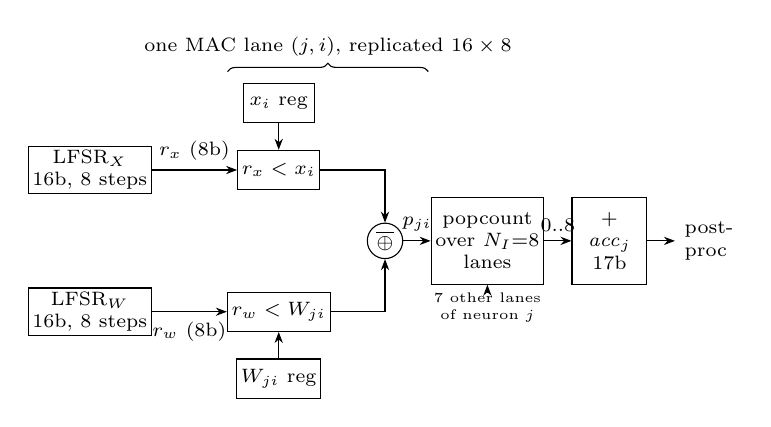
\begin{tikzpicture}[
    font=\scriptsize,
    box/.style={draw, align=center, minimum height=0.5cm, inner sep=1.5pt},
    gate/.style={draw, circle, inner sep=0.5pt, minimum size=0.45cm},
    >={Stealth[length=1.4mm]}]
  % Random number sources
  \node[box, minimum width=1.25cm] (lx) at (-0.2,0.9) {LFSR$_X$\\16b, 8 steps};
  \node[box, minimum width=1.25cm] (lw) at (-0.2,-0.9) {LFSR$_W$\\16b, 8 steps};
  % Comparators of lane (j,i)
  \node[box] (cx) at (2.2,0.9) {$r_x<x_i$};
  \node[box] (cw) at (2.2,-0.9) {$r_w<W_{ji}$};
  \node[box, minimum width=0.9cm] (xr) at (2.2,1.75) {$x_i$ reg};
  \node[box, minimum width=0.9cm] (wr) at (2.2,-1.75) {$W_{ji}$ reg};
  \draw[->] (lx) -- node[above]{$r_x$ (8b)} (cx);
  \draw[->] (lw) -- node[below]{$r_w$ (8b)} (cw);
  \draw[->] (xr) -- (cx);
  \draw[->] (wr) -- (cw);
  % XNOR
  \node[gate] (xn) at (3.55,0) {$\overline{\oplus}$};
  \draw[->] (cx.east) -| (xn.north);
  \draw[->] (cw.east) -| (xn.south);
  % Popcount and accumulator
  \node[box, minimum width=1.15cm, minimum height=1.1cm] (pc) at (4.85,0)
       {popcount\\over $\IL{=}8$\\lanes};
  \draw[->] (xn) -- node[above]{$p_{ji}$} (pc);
  \node[font=\tiny, align=center] at (4.85,-0.85) {7 other lanes\\of neuron $j$};
  \draw[->] (4.85,-0.65) -- (pc.south);
  \node[box, minimum width=0.95cm, minimum height=1.1cm] (acc) at (6.4,0)
       {$+$\\$\mathit{acc}_j$\\17b};
  \draw[->] (pc) -- node[above]{0..8} (acc);
  \draw[->] (acc.east) -- ++(0.35,0) node[right, align=left]{post-\\proc};
  % Replication brace
  \draw[decorate, decoration={brace, amplitude=3pt}]
       (1.55,2.15) -- (4.1,2.15) node[midway, above=2pt]
       {one MAC lane $(j,i)$, replicated $16\times 8$};
\end{tikzpicture}
\caption{One MAC lane of the SC tile and the APC of neuron $j$. The input
comparator $[r_x<x_i]$ is shared by the 16 neuron lanes; every weight has its
own comparator. In RNG mode 1 lane $i$ uses $\mathrm{rotl}_8(r,i)$; in mode 2
each input lane has its own LFSR pair.}
\label{fig:tile}
\end{figure}

\subsection{Leap-forward LFSR and RNG modes}
All generators are 16-bit Fibonacci LFSRs with the polynomial
$x^{16}+x^{14}+x^{13}+x^{11}+1$ (period 65535, maximal, \lbl{calculation}).
% evidence: design/architecture/ARCHITECTURE.md sec. 5.3; requirements/BUDGETS.md sec. 9 (scripts/budgets/logs/lfsr_check.log)
To avoid the shifted-copy correlation of consecutive single-step outputs, each
stream cycle advances every LFSR by \emph{eight} steps and uses the low byte of
the new state as $r$ (ADR-005). Symbolic expansion over GF(2) shows that each
of the eight new bits is the XOR of exactly four current-state bits while the
other eight bits are a plain shift, so the leap costs eight LUT4s and one
logic level per LFSR (\lbl{calculation}).
% evidence: requirements/BUDGETS.md sec. 1.2 (8-step leap-forward); management/DECISIONS.md ADR-005
The golden model verifies the unrolled network against eight single steps for
all 65536 states.
% evidence: management/handoffs/software-engineer/SW-01a.md (test_leap8_equals_8_single_steps_for_all_states, logs/sw/pytest_model.log)

Three RNG modes are a synthesis parameter (ADR-003):
\begin{itemize}
\item \emph{Mode 0 (shared)}: one LFSR$_X$ (seed \texttt{0xACE1}) for all
  input lanes and one LFSR$_W$ (seed \texttt{0x7A5C}) for all weight lanes.
\item \emph{Mode 1 (rotate)}: the same two LFSRs, lane $i$ uses
  $\mathrm{rotl}_8(r,i)$, a free re-wiring.
\item \emph{Mode 2 (independent)}: one LFSR pair per input lane, seeds
  $(\texttt{0xACE1}+\texttt{0x3C5A}\,i)\bmod 2^{16}$ and
  $(\texttt{0x7A5C}+\texttt{0x2B67}\,i)\bmod 2^{16}$, shared by the 16 neuron
  lanes.
\end{itemize}
% evidence: design/architecture/ARCHITECTURE.md sec. 5.3 RNG_MODE
The LFSRs are loaded with their seeds when START is accepted, advance only in
stream cycles and are not reset between tiles or layers. In a pre-RTL
calibration benchmark of one tile, mode 2 cost 112 LUT4 and 224 flip-flops more
than modes 0/1 (\lbl{simulation} of synthesis and place-and-route).
% evidence: requirements/BUDGETS.md sec. 1.2 table (scripts/budgets/logs/ubench_run1.log)
The rev~A default is mode 1. A design revision (rev~B) that makes mode 2 the
default and re-spaces its seeds is in progress; its seeds are \TBD{revB-seeds}.
% evidence: management/DECISIONS.md ADR-003 (default mode 1); task statement DOC-01 (rev B announced)

\subsection{Post-processing (bit-exact)}
After the last tile of a layer each neuron $j$ is post-processed with integer
arithmetic exactly as in the specification (rev~A, Sec.~5.3), with $N_{in}$
the layer fan-in, $K\in\{4,\dots,10\}$ and the activation shift
$s\in\{0,\dots,7\}$:
\begin{align}
  D_j &= 2\,\mathit{acc}_j - N_{in}L, \label{eq:D}\\
  B_j &= \left\lfloor \mathit{bias}_j\, 2^K / 128 \right\rfloor,
  \qquad \Dp_j = D_j + B_j, \label{eq:B}\\
  u_j &= \left\lfloor \Dp_j\, 2^{s+7} / 2^K \right\rfloor, \nonumber\\
  \mathrm{HIDDEN}_j &= 128 + \mathrm{clip}(u_j,0,127), \label{eq:hidden}\\
  \mathrm{SCORE}_j &= \Dp_j \;\text{(signed, 32 bits)}, \label{eq:score}
\end{align}
where \eqref{eq:hidden} applies to layer~1 (hidden codes),
\eqref{eq:score} to layer~2, $\mathit{bias}_j$ is a signed 16-bit integer in
units of $1/128$, and
$\mathrm{RESULT}=\arg\max_{j\in\{0..9\}}\mathrm{SCORE}_j$ with ties resolved to
the lowest index. Since $E[\overline{a\oplus b}]=(1+v_av_b)/2$,
$\Dp_j/L$ is an unbiased estimate of $\sum_i v(x_i)v(W_{ji})+\mathit{bias}_j/128$
up to the floor in $B_j$.
% evidence: design/architecture/ARCHITECTURE.md sec. 5.3 (post-process, interpretation)
The accumulator needs 17 unsigned bits and $\Dp$ 20 signed bits; the product
$\Dp\,2^{s+7}$ reaches about $2^{32.3}$ and is therefore implemented as a
saturating shift rather than a multiplication (\lbl{calculation}).
% evidence: requirements/BUDGETS.md sec. 1.3 (logs/stats_budget.log); reports/sw/accuracy.json value_ranges

\subsection{Programming model and tile schedule}
Weights and biases are written once through the bus into the weight RAM and the
BIAS buffer. Per inference the CPU writes the 64 input codes (16 words), sets
LOG2\_L and ACT\_SHIFT in CONFIG, writes START, polls STATUS.DONE and reads
RESULT; the CYCLES register reports the busy time.
% evidence: design/architecture/ARCHITECTURE.md sec. 5.4, 8
Fig.~\ref{fig:timing} shows the schedule of a tile as assumed by the latency
budget: 32 word reads from the weight RAM, one cycle of BSRAM latency and three
cycles to load the inputs, then $L$ stream cycles; after the last tile of a
layer, 16 cycles of post-processing (one neuron per cycle) and 2 cycles of
clear/drain.
% evidence: requirements/BUDGETS.md sec. 3 (O_TILE = 36, P_POST = 16, C_LAYER = 2: ASSUMPTION)
The cycle-accurate schedule of the RTL is \TBD{tpu-tile-schedule}.

\begin{figure}[!t]
\centering
\resizebox{\columnwidth}{!}{%
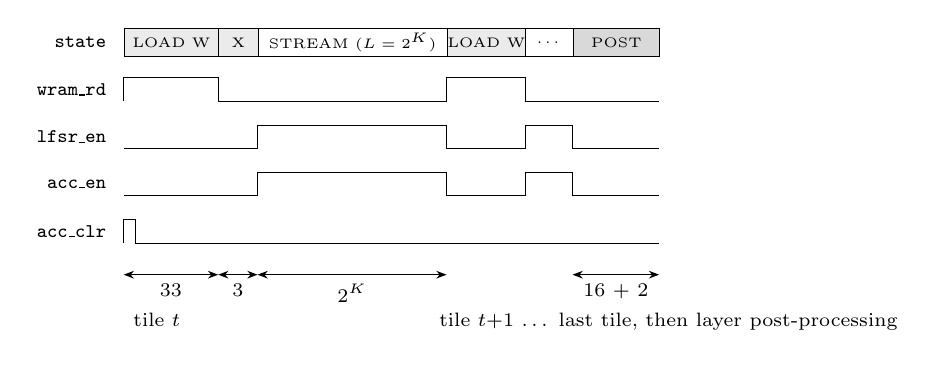
\begin{tikzpicture}[font=\scriptsize, >={Stealth[length=1.3mm]},
    seg/.style={draw, minimum height=0.36cm, inner sep=0pt, anchor=west,
                align=center}]
  % Signal names
  \foreach \y/\n in {0/state, -0.6/wram\_rd, -1.2/lfsr\_en, -1.8/acc\_en,
                     -2.4/acc\_clr}
    \node[anchor=east] at (-0.1,\y) {\texttt{\n}};
  % State bar (not to scale)
  \node[seg, minimum width=1.2cm, fill=black!8, font=\tiny] at (0,0) {LOAD W};
  \node[seg, minimum width=0.5cm, fill=black!8, font=\tiny] at (1.2,0) {X};
  \node[seg, minimum width=2.4cm, font=\tiny] at (1.7,0) {STREAM ($L=2^K$)};
  \node[seg, minimum width=1.0cm, fill=black!8, font=\tiny] at (4.1,0) {LOAD W};
  \node[seg, minimum width=0.6cm, font=\tiny] at (5.1,0) {\dots};
  \node[seg, minimum width=1.1cm, fill=black!15, font=\tiny] at (5.7,0) {POST};
  % wram_rd high during LOAD W
  \draw (0,-0.75) -- (0,-0.45) -- (1.2,-0.45) -- (1.2,-0.75) -- (4.1,-0.75)
        -- (4.1,-0.45) -- (5.1,-0.45) -- (5.1,-0.75) -- (6.8,-0.75);
  % lfsr_en and acc_en high during STREAM
  \foreach \y in {-1.2,-1.8}{
    \draw (0,\y-0.15) -- (1.7,\y-0.15) -- (1.7,\y+0.15) -- (4.1,\y+0.15)
          -- (4.1,\y-0.15) -- (5.1,\y-0.15) -- (5.1,\y+0.15) -- (5.7,\y+0.15)
          -- (5.7,\y-0.15) -- (6.8,\y-0.15);}
  % acc_clr pulse at layer start
  \draw (-0.0,-2.55) -- (0,-2.25) -- (0.15,-2.25) -- (0.15,-2.55) -- (6.8,-2.55);
  % Durations
  \draw[<->] (0,-2.95) -- node[below]{33} (1.2,-2.95);
  \draw[<->] (1.2,-2.95) -- node[below]{3} (1.7,-2.95);
  \draw[<->] (1.7,-2.95) -- node[below]{$2^K$} (4.1,-2.95);
  \draw[<->] (5.7,-2.95) -- node[below]{16 + 2} (6.8,-2.95);
  \node[anchor=west, align=left] at (0,-3.55)
       {tile $t$ \hspace{3.1cm} tile $t{+}1$ \dots\ last tile, then layer post-processing};
\end{tikzpicture}}
\caption{Tile schedule of the latency budget (durations in clock cycles,
\lbl{assumption}: $O_{\mathrm{tile}}=32{+}1{+}3=36$ load cycles per tile,
$16+2$ cycles per layer for post-processing and clear). The LFSRs advance only
while \texttt{lfsr\_en} is high. Not to scale; RTL schedule \TBD{tpu-tile-schedule}.}
% evidence: requirements/BUDGETS.md sec. 3
\label{fig:timing}
\end{figure}

% =============================================================================
\section{Co-Design and Verification Methodology}
\label{sec:method}

\subsection{Bit-exact golden model}
The Python golden model implements the specification twice: a literal
reference with explicit loops and eight single LFSR steps per stream cycle,
and a vectorised engine that pre-computes, per tile and lane, a count table
from the histogram of $(r_x,r_w)$ pairs, which makes the 360-image accuracy
sweeps fast. The two agree on 16 random cases per mode for $K=4..10$ including
extreme codes and biases, and the exported test vectors (257 vectors
$\times$ 33 fields: hidden codes, scores, result) were regenerated by the
reference model with 0 mismatches (\lbl{simulation}).
% evidence: logs/sw/gen_hex.log ("CROSSCHECK TOTAL: 257 vectors x 33 fields, mismatches = 0"); logs/sw/pytest_model.log ("33 passed")
For the RTL testbench the model exports 360 vectors per RNG mode at $K=8$,
additional vectors at $K=4$ and $K=10$, corner-case parameter sets and
cycle-by-cycle RNG traces. The RTL-versus-model comparison is
\TBD{tpu-bitexact-mismatches} mismatches over \TBD{tpu-vectors-total} vectors.
% evidence: management/handoffs/software-engineer/SW-01a.md (outputs: sim/data/tpu_vectors_*.txt)

\subsection{Training with SC noise}
The data set is the 8$\times$8 handwritten-digits set distributed with
scikit-learn~\cite{pedregosa2011sklearn,uci_digits} (1797 images, pixels
0..16). A stratified split gives 1437 training and 360 test images; 288 of the
training images form a validation split used for every model choice, and the
test split is used only for the final numbers. Pixels map to codes
$c=128+\lfloor(127p+8)/16\rfloor$, i.e.\ non-negative bipolar values.
% evidence: reports/sw/accuracy.json "split", "dataset"; code/python/sctpu/train.py pixel_to_code
Three variants were trained (Adam, 300 epochs, straight-through estimator for
the code rounding): \emph{float} (rounded after training), \emph{qat}
(quantisation-aware) and \emph{qat\_noise}, which adds zero-mean Gaussian noise
with the independent-stream variance of~\eqref{eq:var3} at $K=8$ to both
layers' pre-activations during training. The selected model is qat\_noise with
$s=0$, chosen on the validation split.
% evidence: management/handoffs/software-engineer/SW-01a.md (assumptions, selected model); reports/sw/accuracy.json selected_variant, selected_s

\subsection{Analytical error model}
Writing each stream bit as a spin $\sigma=2b-1$ and assuming uniform,
cycle-independent $r$ and independent X and W generators, the variance of the
estimate $\Dp/L$ of one neuron is (\lbl{calculation})
\begin{equation}
  \mathrm{Var}\!\left(\frac{\Dp}{L}\right) = \frac{1}{L}\sum_{\text{tiles}}
  \Big[\sum_{i,k} C^{x}_{ik} C^{w}_{ik} - \Big(\sum_i v_{x,i} v_{w,i}\Big)^2\Big],
  \label{eq:var2}
\end{equation}
where $C_{ik}$ is the spin correlation of lanes $i$ and $k$ within a tile
($C_{ii}=1$). With shared numbers (mode 0) $C_{ik}=1-2|a-b|/256$ for codes $a,b$;
mode 1 is enumerated exactly over the 256 values of $r$; for independent lanes
(mode 2) it reduces to
\begin{equation}
  \mathrm{Var}\!\left(\Dp/L\right) = \frac{1}{L}\sum_i \left(1 - v_{x,i}^2
  v_{w,i}^2\right).
  \label{eq:var3}
\end{equation}
% evidence: reports/sw/error_model.md eqs. (1)-(3)
Two consequences follow. The variance is largest for zero products; since most
digit pixels are blank (code 128), layer~1 operates close to its worst case
$64/L$. Sharing random numbers makes lanes with similar codes almost perfectly
correlated and can multiply the variance by up to $\IL=8$.

\subsection{CPU verification by ISS-based differential testing}
CPU stimuli are produced by a Python reference assembler and checked on a
Python instruction-set simulator (ISS); they are testbench stimuli, not
firmware. The suite has 44 programs: 11 directed, 20 random (200-instruction
bodies, recorded seeds) and 13 trap tests covering every trap cause. Each
program ends by dumping all registers into a 32-word signature. The ISS and
assembler are covered by 93 unit tests, including hand-derived encodings and an
assemble/disassemble round trip over 48\,502 seeded instruction words with 0
mismatches.
% evidence: management/handoffs/software-engineer/SW-01b.md; logs/sw/pytest_rv32.log ("93 passed"); reports/sw/cpu_tests_summary.json
The self-checking RTL testbench runs every program under four bus timings
(0, 1 and 3 wait states, and random 0--7 cycle stalls) and compares the
signature, stop kind, trap cause, halt PC, retired-instruction count, TOHOST
value, bus-error flag, LED and UART output with the ISS. A bus-protocol checker
enforces seven rules (stable requests while waiting, no ready without valid,
no X/Z, aligned fetches, exact byte strobes, one data access per instruction,
silence after halt).
% evidence: management/handoffs/fpga-engineer/RTL-CPU.md (checks, protocol checker rules P1-P7)

\subsection{Fault injection}
A passing testbench proves little unless it can fail. Every testbench is
therefore re-run with an injected fault and must report failure: for the CPU,
a corrupted expected signature and a request that changes while waiting for
\texttt{mem\_ready} both produce \texttt{TEST FAILED} with a non-zero exit
code; the test generator itself is checked by a deliberately wrong expected
value. The SC-TPU testbench fault-injection result is \TBD{tpu-tb-faultinj}.
% evidence: logs/cpu/sim_cpu_summary.log ("negative checks: sig fault -> TEST FAILED ... proto fault -> TEST FAILED"); requirements/REQUIREMENTS.md REQ-VER-002

\subsection{Open-source implementation flow}
Synthesis uses Yosys~0.70 with the Gowin script and wide-function
multiplexers disabled (option \texttt{-nowidelut}); placement and routing use
nextpnr-0.11.1 (himbaechel back end, family GW1N-9C, 27\,MHz constraint), and the
bitstream is packed with Apicula~0.32 only as a proof of routability; it was
never programmed into a device. Simulation uses Icarus Verilog
12.0~\cite{icarus} and lint Verilator 5.020~\cite{verilator}.
% evidence: reports/fpga/cpu/cpu_synth_pnr.txt (tool header); management/TOOLCHAIN.md
Each design is placed and routed with three seeds and the \emph{worst}
post-route Fmax is reported. The acceptance targets are Fmax $\ge 29.7$\,MHz
(27\,MHz + 10\,\%) and at most 85\,\% of each device resource.
% evidence: design/architecture/ARCHITECTURE.md sec. 10 (rev A.2 margins)

% =============================================================================
\section{Results}
\label{sec:results}
All results in this section are \lbl{simulation} (golden model, RTL
simulation or static timing analysis of the place-and-route result) or
\lbl{calculation}; none is a hardware measurement.

\subsection{Accuracy versus stream length and RNG mode}
Fig.~\ref{fig:acc} and Table~\ref{tab:acc} give the test accuracy of the
bit-exact model with the rev~A hardware seeds and, as a check that one seed set
is not a lucky or unlucky draw, the mean over 16 analysis-only LFSR start
offsets. The reference is the expected-value (EV) model, in which every stream
is replaced by its expectation: 95.0\,\% (342/360, CI 92.2--96.8\,\%). An exact
int8 binary datapath on the same codes gives the identical result (0 mismatches
in hidden codes, scores and results), so it serves as the non-SC baseline.
% evidence: reports/sw/accuracy.json models.qat_noise.expected_value_Kinf, int8_binary, int8_vs_ev_mismatches_hidden_score_result
For comparison, a float-trained network evaluated in floating point reaches
96.1\,\% (346/360).
% evidence: reports/sw/accuracy.json float_trained_at_hw_s

\begin{figure}[!t]
\centering
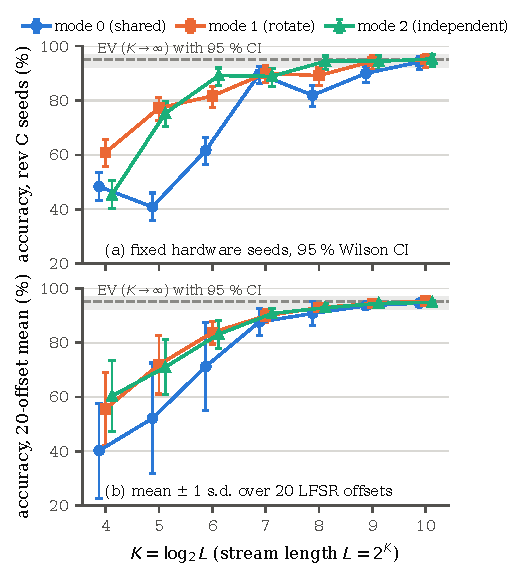
\includegraphics[width=\columnwidth]{article_acc_vs_k.pdf}
\caption{Test accuracy ($n=360$) of the bit-exact model versus $K$ for the
three RNG modes (\lbl{simulation}). (a) Rev~A hardware seeds with 95\,\% Wilson
intervals; (b) mean $\pm$ one standard deviation over 16 LFSR start offsets.
Grey: EV model with its 95\,\% interval. Data: \texttt{reports/sw/accuracy.json}.}
% evidence: reports/sw/accuracy.json; generator reports/figures/article_figures.py; log logs/doc/article_figures.log
\label{fig:acc}
\end{figure}

\begin{table*}[!t]
\centering
\caption{Test accuracy [\%] versus $K$ (\lbl{simulation}, golden model,
selected model qat\_noise, $s=0$, $n=360$). HW: rev~A hardware seeds, correct
count $k$ and 95\,\% Wilson CI; Ens.: mean $\pm$ s.d.\ over 16 LFSR start
offsets. EV ($K\to\infty$): 95.0 (342/360, CI 92.2--96.8).}
\label{tab:acc}
% evidence: reports/sw/accuracy.json models.qat_noise.sc and .sc_ensemble_accuracy (printed in logs/doc/article_figures.log)
\setlength{\tabcolsep}{4.2pt}
\begin{tabular}{@{}c|ccc|ccc|ccc@{}}
\toprule
 & \multicolumn{3}{c|}{Mode 0 (shared)} & \multicolumn{3}{c|}{Mode 1 (rotate)} & \multicolumn{3}{c}{Mode 2 (independent)}\\
$K$ & HW ($k$) & CI & Ens. & HW ($k$) & CI & Ens. & HW ($k$) & CI & Ens.\\
\midrule
4  & 58.6 (211) & 53.5--63.6 & 41.9$\pm$17.6 & 63.6 (229) & 58.5--68.4 & 56.3$\pm$11.7 & 45.3 (163) & 40.2--50.4 & 59.6$\pm$13.9\\
5  & 41.4 (149) & 36.4--46.5 & 54.4$\pm$20.1 & 66.4 (239) & 61.4--71.1 & 68.7$\pm$10.7 & 75.3 (271) & 70.6--79.5 & 70.8$\pm$10.2\\
6  & 65.3 (235) & 60.2--70.0 & 65.2$\pm$18.3 & 84.2 (303) & 80.0--87.6 & 86.5$\pm$4.6 & 89.2 (321) & 85.5--92.0 & 84.5$\pm$4.5\\
7  & 49.7 (179) & 44.6--54.9 & 81.6$\pm$13.4 & 92.2 (332) & 89.0--94.6 & 90.1$\pm$2.6 & 88.9 (320) & 85.2--91.7 & 90.5$\pm$1.6\\
8  & 65.6 (236) & 60.5--70.3 & 89.7$\pm$6.2 & 91.1 (328) & 87.7--93.6 & 93.3$\pm$1.9 & 94.4 (340) & 91.6--96.4 & 92.7$\pm$1.5\\
9  & 88.6 (319) & 84.9--91.5 & 93.7$\pm$1.2 & 94.7 (341) & 91.9--96.6 & 94.4$\pm$1.0 & 94.4 (340) & 91.6--96.4 & 94.4$\pm$0.6\\
10 & 94.4 (340) & 91.6--96.4 & 94.5$\pm$0.8 & 94.7 (341) & 91.9--96.6 & 95.1$\pm$0.6 & 95.3 (343) & 92.6--97.0 & 94.8$\pm$0.5\\
\bottomrule
\end{tabular}
\end{table*}

Three observations follow. First, decorrelation matters more than stream
length at moderate $K$: at the reset default $K=8$ ($L=256$) the hardware
seeds give 65.6\,\% with shared numbers, 91.1\,\% with rotation and
94.4\,\% with independent generators. Second, the smallest $K$ at which the
hardware-seed accuracy stays within 1 percentage point (pp) of EV for all
larger $K$ is 10, 9 and 8 for modes 0, 1 and 2; with the ensemble mean it is
10, 9 and 9. Third, mode~0 is non-monotonic in $K$ (49.7\,\% at $K=7$,
65.6\,\% at $K=8$) although its ensemble mean rises monotonically (81.6\,\% and
89.7\,\%): with one shared generator pair all images see the same few
empirical $(r_x,r_w)$ histograms, so one seed set has few degrees of freedom.
% evidence: reports/sw/accuracy.json design_rule, design_rule_ensemble_mean, sc, sc_ensemble_accuracy; reports/sw/error_model.md (measurement paragraph)
Note that 1\,pp corresponds to 3.6 images, well below the 95\,\% CI half-width of
2.3--3.1\,pp for accuracies between 95 and 90\,\%; in particular the 2-image gap between mode~2 at
$K=8$ (340/360) and EV (342/360) is not statistically resolved.
% evidence: reports/sw/accuracy.json ci95 (mode2 K8: 91.6-96.4); requirements/BUDGETS.md sec. 8
Noise-aware training did not change the $s=0$ result significantly (mode~2,
$K=8$: 95.3\,\% for qat versus 94.4\,\% for qat\_noise), but post-training
rounding of a float-trained model did not reach EV$-$1\,pp for any $K\le10$.
% evidence: reports/sw/accuracy.json models.qat.sc["2"]["8"] = 343/360, models.float.design_rule = None; management/handoffs/software-engineer/SW-01a.md
The rev~B seeds will change the mode-2 hardware-seed row; its $K=8$ value is
\TBD{acc-revB-mode2-K8}.

\subsection{Error model versus simulation}
Fig.~\ref{fig:rms} compares the RMS error of $\Dp/L$ (deterministic bias term
removed) with~\eqref{eq:var2}. Over the 16-offset ensemble the ratio of
measured to predicted RMS lies within 0.82--1.13 for 41 of the 42
layer/$K$/mode combinations; the exception is mode~0, layer~1, $K=10$ (0.74).
The prediction tracks the $1/\sqrt{L}$ law and the penalty of mode~0
(at $K=8$, layer~1: 0.82 measured, 0.79 predicted, versus 0.50/0.48 for
mode~2). A single hardware-seed realisation can deviate much more: 1.55 for
mode~0 at $K=8$, a factor 1.96 above the prediction, which explains the
mode-0 accuracy dips.
% evidence: reports/sw/error_model.md (agreement paragraph, table); reports/sw/accuracy.json error_study.per_mode_K
The model treats different stream cycles as independent. All LFSRs, however,
run on the same maximal-length sequence: with the 8-step leap, two generators
whose seeds are $d$ single steps apart produce the same numbers with a lag of
$d\cdot 8^{-1} \bmod 65535$ stream cycles. In rev~A mode~2 the smallest such
lag is 321 cycles (X$_0$/W$_3$), i.e.\ inside one layer from $K=6$; the
ensemble agreement for mode~2 (0.89--1.06) suggests a small effect.
% evidence: reports/sw/error_model.md (known limitations); reports/sw/accuracy.json lfsr_lags
At $K=10$ an inference uses $1.25$ LFSR periods, so the sequence wraps within
one inference (\lbl{calculation}).
% evidence: requirements/BUDGETS.md sec. 9 (scripts/budgets/logs/lfsr_check.log)

\begin{figure}[!t]
\centering
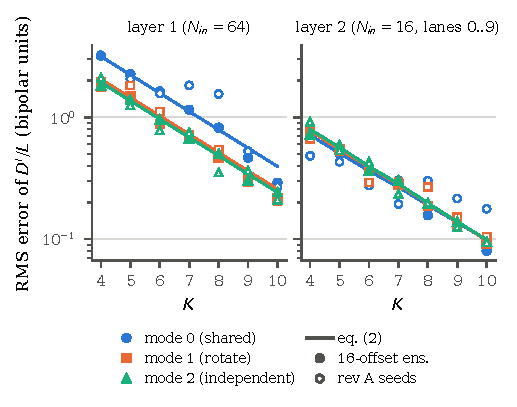
\includegraphics[width=\columnwidth]{article_rms_vs_k.pdf}
\caption{RMS stochastic error of $\Dp/L$ per neuron versus $K$
(\lbl{simulation} and \lbl{calculation}): ensemble measurement (filled),
prediction~\eqref{eq:var2} (lines) and the single rev~A hardware-seed
realisation (open). Layer 2 uses the SC hidden codes of the same run.}
% evidence: reports/sw/accuracy.json error_study; generator reports/figures/article_figures.py
\label{fig:rms}
\end{figure}

\subsection{Latency and throughput}
With the tile schedule of Fig.~\ref{fig:timing}, an inference takes
(\lbl{calculation}, inputs partly \lbl{assumption})
\begin{equation}
  N(K) = 10\cdot 2^K + 409 \;\text{clock cycles},
  \label{eq:latency}
\end{equation}
i.e.\ ten tiles of $2^K$ stream cycles plus 360 cycles of tile loading and 49
cycles of post-processing, argmax and handshaking.
% evidence: requirements/BUDGETS.md sec. 3 (closed form; known-answer check N(8) = 2969 PASS in scripts/budgets/logs/latency_budget.log)
Table~\ref{tab:latency} pairs the latency with the accuracy of
Table~\ref{tab:acc}. At $K=8$ an inference takes 2969 cycles or
110\,\textmu s at 27\,MHz (9094 inferences/s), of which 86.2\,\% are stream
cycles. The measured CYCLES register value of the RTL is
\TBD{tpu-cycles-K8}; the requirement allows at most $1.10\,N(K)$.
% evidence: requirements/BUDGETS.md sec. 3 table; requirements/REQUIREMENTS.md REQ-TIM-004
The CPU-side overhead per inference (writing inputs, START, polling, reading
RESULT) is \TBD{soc-cpu-overhead-cycles}.

\begin{table}[!t]
\centering
\caption{Latency $N(K)$ (\lbl{calculation}, eq.~\eqref{eq:latency}) at
27\,MHz and accuracy with rev~A hardware seeds (\lbl{simulation})}
\label{tab:latency}
% evidence: requirements/BUDGETS.md sec. 3 (cycles, time, inferences/s); reports/sw/accuracy.json (accuracy)
\setlength{\tabcolsep}{4pt}
\begin{tabular}{@{}rrrrrr@{}}
\toprule
$K$ & $L$ & cycles & time [\textmu s] & inf./s & acc. m1 / m2 [\%]\\
\midrule
4  & 16   & 569   & 21.07  & 47\,452 & 63.6 / 45.3\\
6  & 64   & 1049  & 38.85  & 25\,739 & 84.2 / 89.2\\
8  & 256  & 2969  & 109.96 & 9\,094  & 91.1 / 94.4\\
10 & 1024 & 10649 & 394.41 & 2\,535  & 94.7 / 95.3\\
\midrule
\multicolumn{6}{@{}l}{RTL CYCLES at $K=8$: \TBD{tpu-cycles-K8}}\\
\bottomrule
\end{tabular}
\end{table}

\subsection{CPU results}
All 44 programs pass under all four bus timings (176/176 runs) with zero
protocol violations, and both injected faults are detected
(\lbl{simulation}, Icarus Verilog 12.0). The aggregate CPI over the suite is
4.231 at zero wait states (28\,206 cycles for 6667 instructions), 5.593 with
one wait state (the block-RAM slave of the SoC), 8.317 with three and 9.013
with random stalls. Placed and routed with the 4\,KiB RAM, the core closes at
62.46, 53.26 and 55.74\,MHz for seeds 1--3, i.e.\ 53.26\,MHz worst case, 79\,\%
above the 29.7\,MHz acceptance target (\lbl{simulation}, static timing
analysis). The worst path (18.77\,ns, 9.66\,ns logic and 9.11\,ns routing)
runs from the instruction register through the decoder to the FSM next-state
logic.
% evidence: logs/cpu/sim_cpu_summary.log; management/handoffs/fpga-engineer/RTL-CPU.md (CPI ws1/ws3/rand, critical path); logs/cpu/pnr_s1.log, pnr_s2.log, pnr_s3.log; reports/fpga/cpu/cpu_synth_pnr.txt
The core alone maps to 831 LUTs, 74 carry (ALU) cells, 111 flip-flops and two
block RAMs; with the RAM and wrapper it occupies 957 of 8640 LUT4 positions
(11\,\%) and 4 of 26 block RAMs. A first version with a barrel shifter needed
1212 LUT4 positions plus 463 wide-function multiplexers in the same context,
which motivated the iterative shifter.
% evidence: reports/fpga/cpu/cpu_synth_pnr.txt (sections A, B); management/handoffs/fpga-engineer/RTL-CPU.md (errors/deviations: barrel shifter)

\subsection{Resources and timing}
Table~\ref{tab:res} collects the implementation figures. Before the RTL
existed, a calibration benchmark of one 16$\times$8 tile (weight and input
registers, LFSRs, comparators, XNOR, popcount and 17-bit accumulators) was
synthesised and routed to size the design. It needs 2855 LUT4 positions in
modes 0/1, of which 1758 are carry cells, mostly the 136 eight-bit SNG
comparators; this is about 22 LUT4 per MAC lane, 2.4 times the first estimate.
The bottom-up SoC budget built on it is 5735 LUT4 (66.4\,\%) and 2489
flip-flops (38.4\,\%) (\lbl{calculation}).
% evidence: requirements/BUDGETS.md sec. 1.2, 1.4; management/DECISIONS.md ADR-007
The figures of the actual SC-TPU and of the integrated SoC are pending.

\begin{table*}[!t]
\centering
\caption{Resources (GW1NR-9: 8640 LUT4, 6480 FF, 26 BSRAM) and worst-seed
Fmax. LUT4 counts include carry cells and LUT-RAM positions.}
\label{tab:res}
% evidence: requirements/BUDGETS.md sec. 1.1 (device totals SOURCE S-027/S-028/S-031; counting rule), 1.2 (ubench), 1.4 (budget)
% evidence: reports/fpga/cpu/cpu_synth_pnr.txt (CPU in context, seed 1 utilisation; worst seed 53.26 MHz)
\setlength{\tabcolsep}{6pt}
\begin{tabular}{@{}lrrrrl@{}}
\toprule
Block & LUT4 & FF & BSRAM & Fmax worst seed [MHz] & Label\\
\midrule
CPU + 4\,KiB RAM & 957 & 126 & 4 & 53.26 & \lbl{simulation} (P\&R, 3 seeds)\\
SC tile bench, m0/m1 & 2855 & 1454 & 0 & 52.12 & \lbl{simulation} (P\&R of calibration bench)\\
SC tile bench, m2 & 2967 & 1678 & 0 & 52.98 & \lbl{simulation} (P\&R of calibration bench)\\
SoC budget (m1) & 5735 & 2489 & 3 & -- & \lbl{calculation} (bottom-up budget)\\
\midrule
SC-TPU (RTL) & \TBD{tpu-lut} & \TBD{tpu-ff} & \TBD{tpu-bsram} & \TBD{tpu-fmax} & pending (RTL in progress)\\
SoC (RTL) & \TBD{soc-lut} & \TBD{soc-ff} & \TBD{soc-bsram} & \TBD{soc-fmax-worst} & pending\\
\bottomrule
\end{tabular}
\end{table*}
% Note: the m0/m1 bench Fmax 52.12 MHz is the worst seed of mode 1 (52.36 for mode 0);
% the m2 bench worst seed is 52.98 MHz (requirements/BUDGETS.md sec. 1.2).

% =============================================================================
\section{Discussion and Limitations}
\label{sec:discussion}

\textbf{SC versus binary arithmetic on this device.} The SC tile provides 128
bit-level MAC lanes without using any of the 20 hard multipliers, and its
precision is chosen at run time through CONFIG. Its throughput, however, is
low: at $K=8$ the calculated rate is $1.08\times10^7$ useful MAC/s, whereas the
40 9$\times$9 multipliers of the device clocked at 27\,MHz could in principle
deliver $1.08\times10^9$ int8 MAC/s (\lbl{calculation}, no such design was
built). On this device SC is therefore a study of area, decorrelation and
verification, not a throughput win; its appeal grows where hard multipliers
are absent or energy per operation dominates, which we have not measured.
% evidence: requirements/BUDGETS.md sec. 4 (useful MAC/s at K=8; int8 comparison 40 MULT9X9 x 27 MHz, CALCULATION from S-032)

\textbf{Simulation only.} No bitstream has been loaded into a device and no
quantity in this paper is a hardware measurement. Fmax values come from the
static timing model of nextpnr, whose Gowin delay data are reverse-engineered
and not validated against silicon. No power figure is reported: no open power
model exists for the GW1N family, and the vendor estimator is outside the
open-source flow. A physical validation plan is part of the project
requirements but has not been executed.
% evidence: requirements/BUDGETS.md sec. 5 (timing model not silicon-validated), sec. 6 (power NOT RUN); requirements/REQUIREMENTS.md REQ-VER-009

\textbf{Statistical resolution.} With 360 test images one image is 0.28\,pp
and the 95\,\% interval half-width is 2.3--3.1\,pp for accuracies between 95
and 90\,\%. Differences of 1--2\,pp between modes or between $K=8$ and $K=9$
are not resolved, and the selected operating points should be read as
engineering choices. The seed ensemble uses 16 start offsets; the project
requirement asks for at least 20 (\TBD{ensemble-20-seeds}).
% evidence: requirements/BUDGETS.md sec. 8; requirements/REQUIREMENTS.md REQ-AI-006; reports/sw/accuracy.json sc_ensemble_accuracy n_realisations = 16

\textbf{Seeding.} The accuracy of a fixed seed set differs from the ensemble
mean by up to 24\,pp in mode~0 at $K=8$ and the LFSR lag analysis shows
that seed spacing must be judged in stream cycles after the leap, not in
single steps. Rev~B addresses this for mode~2; its effect is \TBD{acc-revB-mode2-K8}.
% evidence: reports/sw/accuracy.json (mode0 K8: 65.6 HW vs 89.7 ensemble mean); reports/sw/error_model.md (lag formula)

\textbf{Workload and data sources.} The 64-16-10 MLP on 8$\times$8 digits is a
deliberately tiny workload; conclusions about accuracy versus $K$ may not
transfer to larger networks. The Gowin data sheet and memory user guide could
not be opened during this work; device totals were taken from the board
vendor's documentation and the open-source chip database, which agree, while
the block-RAM organisation remains an assumption confirmed only by successful
synthesis.
% evidence: management/SOURCES.md (access status; S-001..S-005 SOURCE; S-006/S-007 ASSUMPTION)

% =============================================================================
\section{Conclusion}
\label{sec:conclusion}
We have specified, modelled and partly implemented a stochastic-computing
tensor unit and an RV32I processor for a 9K-LUT FPGA with a fully open-source
flow. Treating the random-number generators as part of a bit-exact contract
makes the SC datapath verifiable against a golden model and exposes the role of
decorrelation: in simulation, independent per-lane generators (rev~A seeds) reach 94.4\,\%
at $L=256$, within the confidence interval of the 95.0\,\% expected-value
accuracy, while shared generators fall to 65.6\,\%. A closed-form variance
model predicts the stochastic error within a factor 0.74--1.13 and gives a
design rule for the stream length. The CPU is verified against an ISS on 176
program runs and closes timing with a wide margin. Pending items are the SC-TPU
and SoC implementation results (\TBD{tpu-lut}, \TBD{soc-fmax-worst}), the
RTL bit-exactness check (\TBD{tpu-bitexact-mismatches}), the rev~B seed study
and, eventually, measurements on hardware.
% evidence: reports/sw/accuracy.json; reports/sw/error_model.md; logs/cpu/sim_cpu_summary.log; logs/cpu/pnr_s2.log

\bibliographystyle{IEEEtran}
\bibliography{refs}

\end{document}
